\documentclass[modern]{aastex631}
\usepackage{amsmath}
\usepackage{amssymb}
\usepackage{hyperref}
\usepackage{bm}
\usepackage{listings}
\usepackage{graphicx}
\usepackage{float}
\usepackage{soul}
\usepackage{mathtools}

% commands
\newcommand{\TODO}{\texttt{todo}}
\newcommand{\set}[1]{\{\,#1\,\}}
\newcommand{\footlink}[1]{\footnote{\url{#1}}}
\DeclareMathOperator*{\argmax}{arg\,max}
\DeclareMathOperator*{\argmin}{arg\,min}
\let\subsectionautorefname\sectionautorefname
\let\subsubsectionautorefname\sectionautorefname

% no indent
\setlength\parindent{0pt}

% code style
\lstdefinestyle{mystyle}{
    backgroundcolor=\color{white},
    commentstyle=\color{gray!70},
    keywordstyle=\color{Bittersweet},
    stringstyle=\color{RoyalBlue},
    basicstyle=\fontsize{8.5}{13}\fontfamily{DejaVuSansMono-TLF}\selectfont,
    breakatwhitespace=false,         
    breaklines=true,
    rulecolor=\color{black!15},
    numbers=none,
    numberstyle=\fontsize{7}{11}\fontfamily{DejaVuSansMono-TLF}\selectfont\color{gray!50},
    framerule=0pt,
    breakindent=5pt,
    resetmargins=true,
    numbersep=10pt,
    frame=single,
    aboveskip=1em,
    belowskip=1em,
    xleftmargin=6pt,
    framexleftmargin=4pt
}
\lstset{style=mystyle}


\begin{document}

\title{starry 2}

% author info
\author{Lionel J. Garcia}
\author{Soichiro Hattori}
\author{Daniel Foreman-Mackey}
\affiliation{Center for Computational Astrophysics, Flatiron Institute, New York, NY, USA}

\keywords{exoplanet detection methods, stellar activity, time series analysis, gaussian processes regression, computational methods, GPU computing}

\begin{abstract}
\end{abstract}

\section*{Introduction}
tldr: Modeling occultation light curves serve a wide variety of science cases, especially in exoplanetary science. The latest models account for non-uniform surfaces of stars (starry), but given the large dataset available, could be optimized further. We present several optimizations that improve on the starry model.


Stellar light curves and radial velocity models provided an important tool to study exoplanetary systems. At the origin of these models lies the first principles of orbital mechanics, the Kepler equations, and the algorithms used to solve them. On top of that, models like Agol, of occultation light curves extended our capability to study these systems in greater details, using transits. In practice, computing this model and making inference based on these observables has been enabled by the implementation of these models with optimized frameworks and inference tools (pymc3), providing robust implementation of sampling algorithms and other inferrence tools. A good example of this synergy is the development of exoplanet and starry in c++ backed by Pymc3 which enabled major discoveries based on large datasets. With the recent lunch of JWST, we crumble under data. For example, transmission spectra on hundreds of channels, multi-planet systems and a large number of free parameters with their priors. At the same time, machine learning continue to grow, and novel framework appear and lead to application in physics. One of this framework is jax, developped by google, and gaining a huge popularity on the astronomy community. JAX is a hp machine-learning library that pre-compile code to LAX for paralilisation. It allows complex model to be written direclty in python, where usually a lower-level langage like C is preferable, and parallelised on CPU, GPU or any lax-compatible device. Not only it's good because of the higher level syntax of python that made it popular in science. But also because of the capability to run expansive models on GPU, a trend observed in other field of ML and DL where scaling is required.

In this paper, we describe an implementation of the starry formalism in jax, allowing for the inference of a large number of parameters on complex models, exploiting the latest dev in ML machinery.

\newpage
\section{starry}\label{starry}

\section{optimization}\label{optimization}
\subsection{Limb-darkening multiplicative maps}
\subsection{Spherical harmonics rotations}

% tldr: rotating SH involves costly matrices computations. Hence its smart to figure out which one to pre-compute. That what RL did, amd it led to 6 elementary rotations. However, now that we use jax we don't care that much, and we can reduce the all thing to a single rotation that is optimized at compiled time.\\\\

With \textit{starry}, every light curve computation at a given time $t$ involves a rotation of the spherical harmonics basis, from the rest-frame of the star (\autoref{fig:rotation_basis}, left) to its sky-projected orientation (\autoref{fig:rotation_basis}, right), with a final rotation relative to the position of the occulting body (see Figure 2. from \citealt{starry}).
\begin{figure}[H]
    \begin{center}
        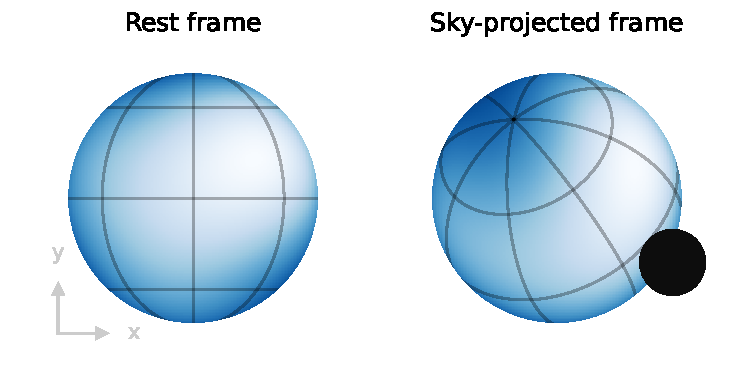
\includegraphics[width=0.6\textwidth]{../workflows/rotations/figures/rotation_basis.pdf}
        \caption{Rotation of the spherical harmonics basis to place the star in the sky-projected frame of the observer.}
        \label{fig:rotation_basis}
    \end{center}
\end{figure}

The rotation of spherical harmonics involves the computation of Wigner-D-matrices, commonly obtained through robust recursion relations in both degree $l$ and order $m$, but leading to costly computations. Hence, knowing how to decompose the full spherical harmonics rotation using pre-computed rotations is essential to achieve optimal performance in the \textit{starry} framework. \autoref{fig:rotation_starry} shows the 6 elementary rotations currently used in the \texttt{starry} implementation.
\begin{figure}[H]
    \begin{center}
        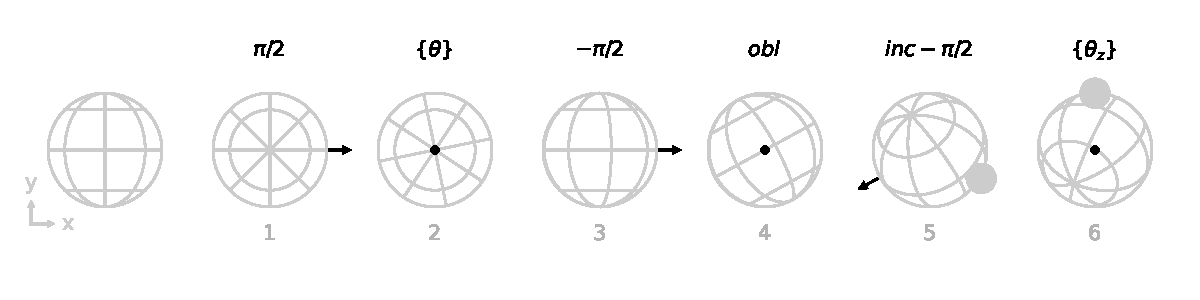
\includegraphics[width=\textwidth]{../workflows/rotations/figures/rotation_starry.pdf}
        \caption{Consecutive rotations of the spherical harmonics basis in the \texttt{starry} implementation. Each schematic shows a sphere rotated from a previous orientation around an axis displayed as a black vector and an angle shown on top.}
        \label{fig:rotation_starry}
    \end{center}
\end{figure}
In this figure, rotations 1 to 3 correspond to a rotation of the star around its rotation axis, and rotations 3 to 5 place the star on a sky-projected frame. Finally, rotation 6 aligns the spherical harmonics map to the occulting body on the $y$ axis in order to apply Green's theorem in the appropriate basis (Figure 2 from \citealt{starry}). The first thing to notice is that rotations 1 to 3 could be simply reduced to a rotation of angle $\theta$ about the y-axis, turning steps 1 to 3 into one. However, rotations around the pole, i.e.\, with a rotation axis along $z$, have simpler expressions that can be implemented separately. In addition, pre-computing these matrices at lower cost is particularly important for steps 2 and 6, involving a potentially large set of angles $\{\theta\}$ and $\{\theta_z\}$, defined over times $\{t\}$, for which to compute the full light curve. This explains the current decomposition of the complete rotation in six separate steps.\\\\
In \texttt{jaxoplanet}, we compute the Wigner-D-matrices by employing the Risbo recursion relations \citep{Risbo1996} implemented in \texttt{JAX} as part of the \texttt{s2fft} Python package \citep{price:s2fft}. In addition, we merge rotations 3, 4 and 5 (see \autoref{fig:rotation_jaxoplanet}) into a single compound rotation of axis
\begin{equation}
    \bm{v} = \frac{1}{\sqrt{1 - \cos^2{\left(\frac{inc}{2} \right)} \cos^2{\left(\frac{obl}{2}\right)}}} \begin{pmatrix}
        \sin{\left(\frac{inc}{2} \right)} \cos{\left(\frac{obl}{2}\right)}\\
        \sin{\left(\frac{inc}{2} \right)} \sin{\left(\frac{obl}{2}\right)}\\
         - \cos{\left(\frac{inc}{2} \right)} \sin{\left(\frac{obl}{2}\right)}\\
    \end{pmatrix},
\end{equation}
and angle
\begin{equation}
    \omega = 2 \cos^{-1}{\left(\cos{\left(\frac{inc}{2} \right)} \cos{\left(\frac{obl}{2}\right)} \right)}.
\end{equation}
This way, the complete rotation reduces to the four separate steps shown in \autoref{fig:rotation_jaxoplanet}.
\begin{figure}[H]
    \begin{center}
        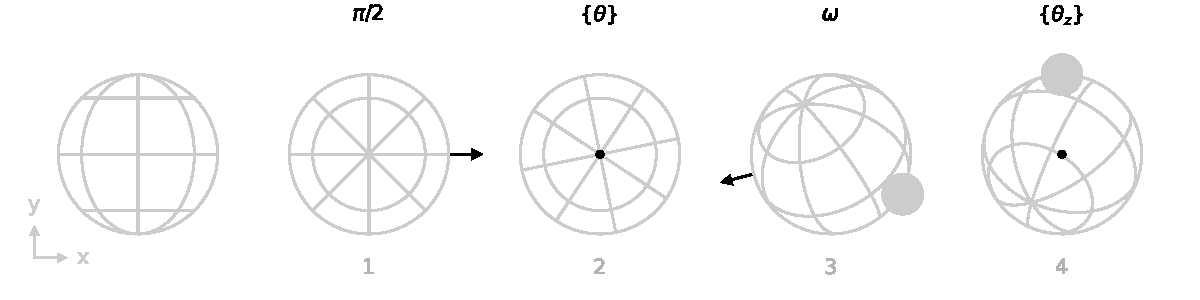
\includegraphics[width=\textwidth]{../workflows/rotations/figures/rotation_jaxoplanet_1.pdf}
        \caption{Consecutive rotations of the spherical harmonics basis in the \texttt{jaxoplanet} implementation. Each schematic shows a sphere rotated from a previous orientation around an axis displayed as a black vector and an angle shown on top.}
        \label{fig:rotation_jaxoplanet}
    \end{center}
\end{figure}

\subsection{Wigner-D matrices}
\subsection{Numerical integration of the solution vectors}

\section{performance}\label{performances}

\section{Case study: ...}

\bibliography{ref}

\end{document}